% \subsection{Motivation}

\begin{frame}{Echo-aware signal processing for \alert{audio scene} analysis}

    Current Scenario

    \begin{columns}[T,onlytextwidth]
        \begin{column}{0.65\textwidth}
            \begin{figure}
                \includegraphics<1>[width=\textwidth]{figures/scene1.png}%
                \includegraphics<2>[width=\textwidth]{figures/scene2.png}%
                \includegraphics<3>[width=\textwidth]{figures/scene3.png}%
                \includegraphics<4>[width=\textwidth]{figures/scene4.png}%
                \includegraphics<5->[width=\textwidth]{figures/scene5.png}%
            \end{figure}
        \end{column}
        \begin{column}{0.34\textwidth}
            \textbf{Sound}
            \begin{itemize}
                \item<1-> produced by \alert{sources}
                \item<2-> recorded by (array of) \alert{microphones}
                \item<3-> corrupted by \alert{noise}
                \item<4-> propagates in the \alert{space}
                \item<5-> interacts with the \alert{room}
                          \\$\hookrightarrow$ \alert{reverberation}
            \end{itemize}
        \end{column}
    \end{columns}

\end{frame}

\begin{frame}[t]{Echo-aware signal processing for \alert{audio scene} analysis}


    \begin{columns}
        \visible<1->{
        \begin{column}[t]{0.3\textwidth}
            \centering
            \alert{Semantic} information

            \vspace*{0.5em}
            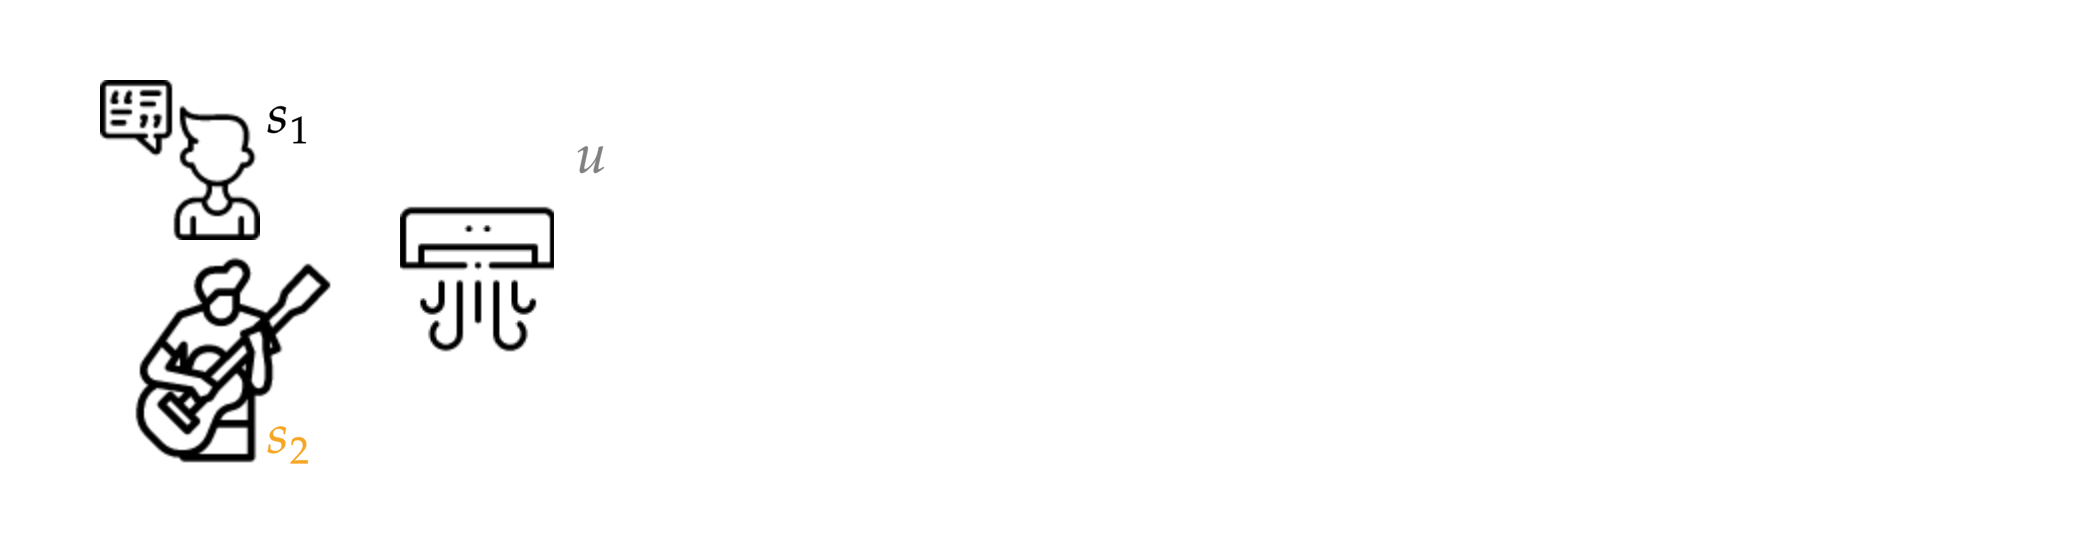
\includegraphics[trim={0 0 170em 0},clip,width=0.5\textwidth]{figures/semantic.png}
        \end{column}}
        \visible<2->{
        \begin{column}[t]{0.3\textwidth}
            \centering
            \alert{Spatial} information

            \vspace*{0.5em}
            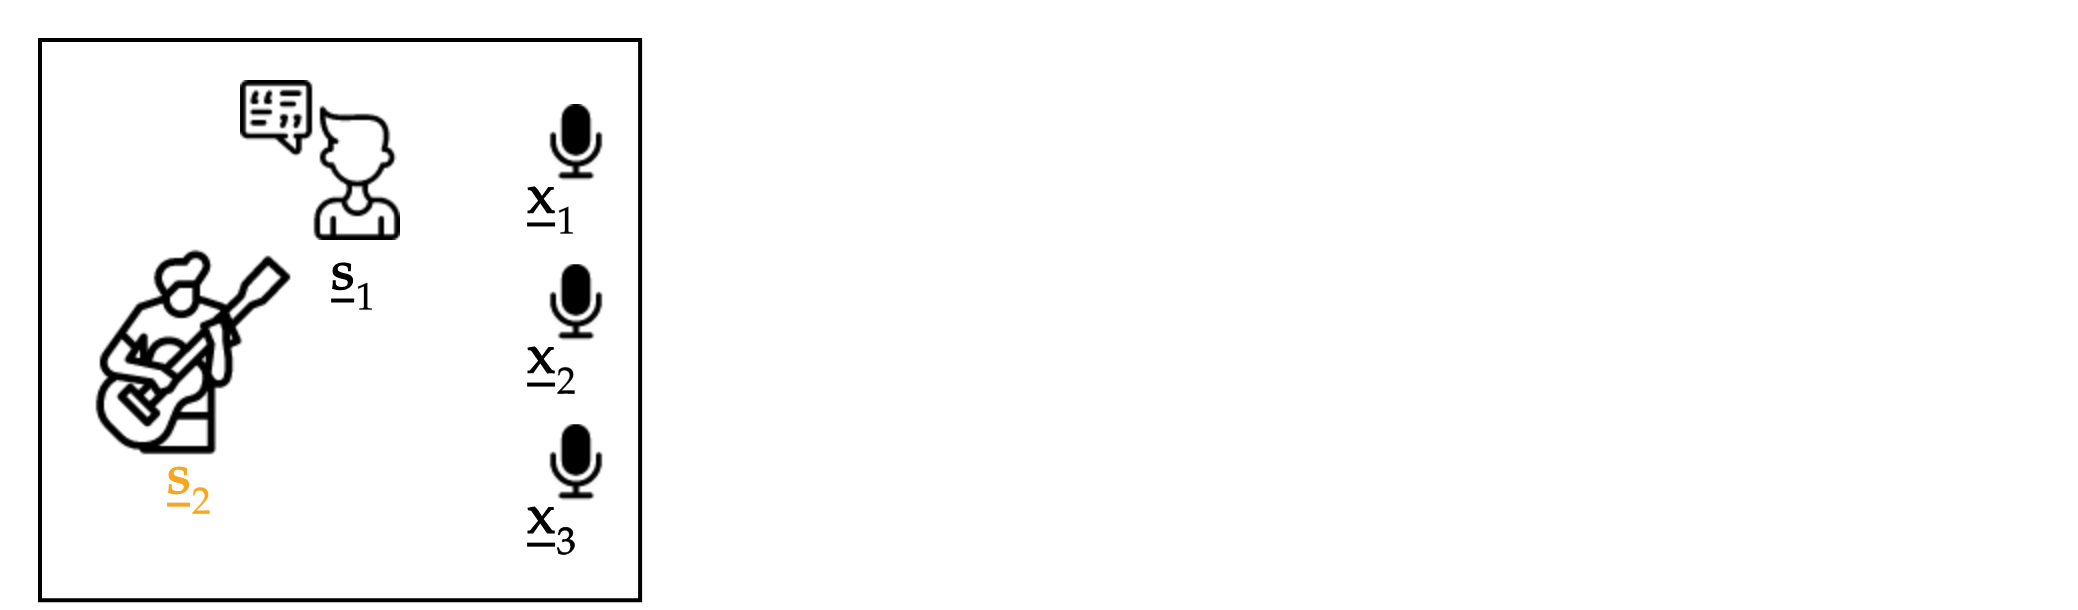
\includegraphics[trim={0 0 170em 0},clip,width=0.5\textwidth]{figures/spatial.png}
        \end{column}}
        \visible<3->{
        \begin{column}[t]{0.3\textwidth}
            \centering
            \alert{Temporal} information

            \vspace*{0.5em}
            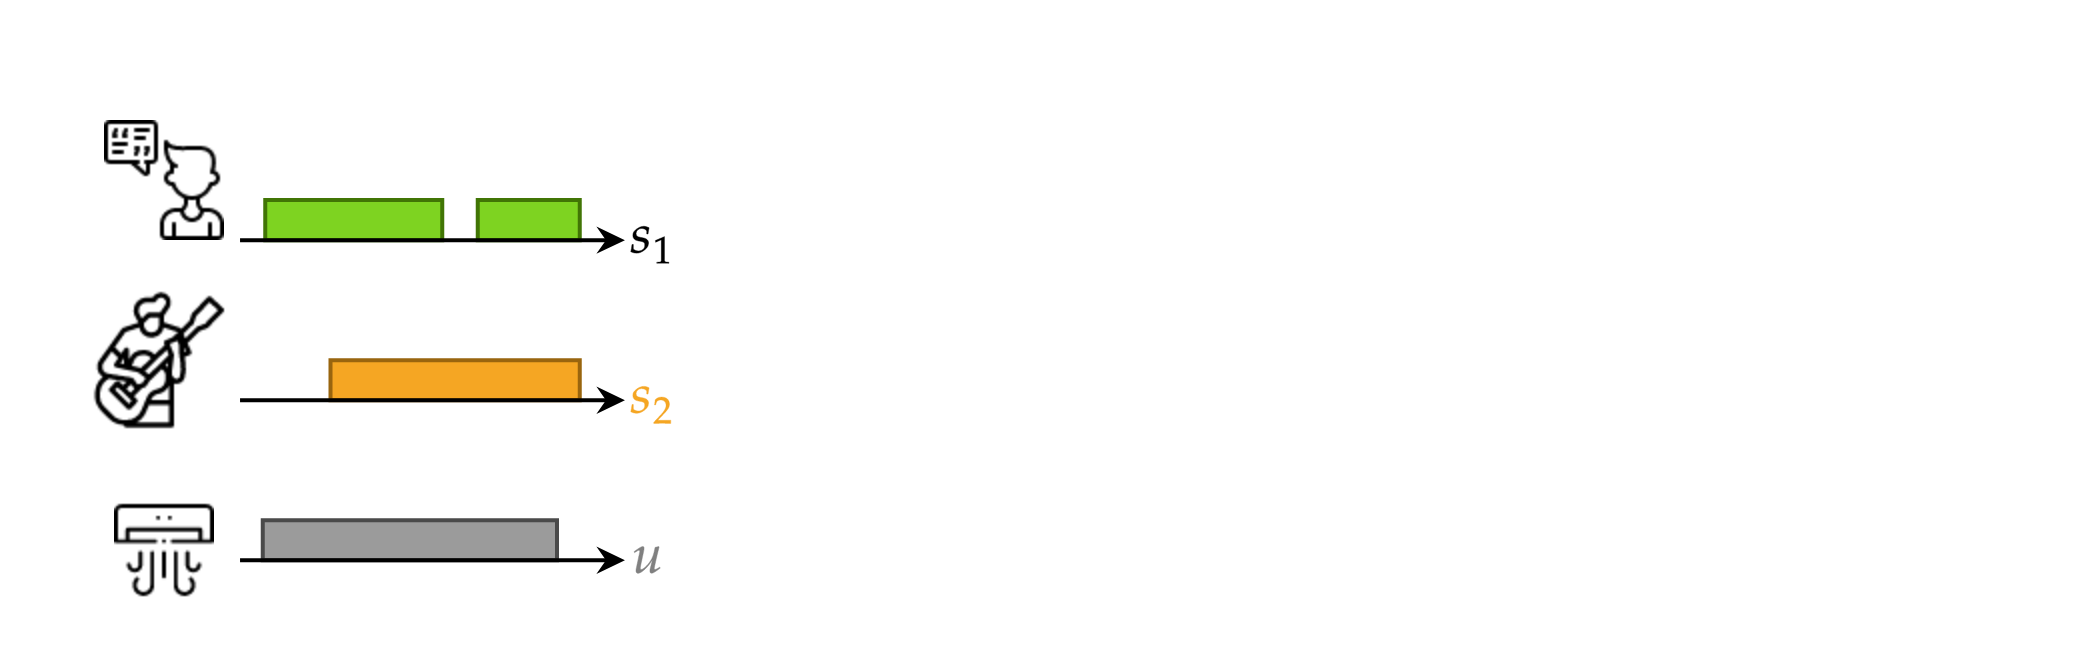
\includegraphics[trim={0 0 170em 0},clip,width=0.5\textwidth]{figures/temporal.png}
        \end{column}}
    \end{columns}

    \begin{columns}
        \visible<1->{
        \begin{column}[t]{0.3\textwidth}
            \centering
            on nature and content
        \end{column}}
        \visible<2->{
        \begin{column}[t]{0.3\textwidth}
            \centering
            on position and geometry
        \end{column}}
        \visible<3->{
        \begin{column}[t]{0.3\textwidth}
            \centering
            on events activity
        \end{column}
        }
    \end{columns}


    \vfill
    \visible<4->{
    \begin{mydefblock}{Audio Scene Analysis}
        Extraction and organization of all the information in the sound
    \end{mydefblock}

    \begin{center}
        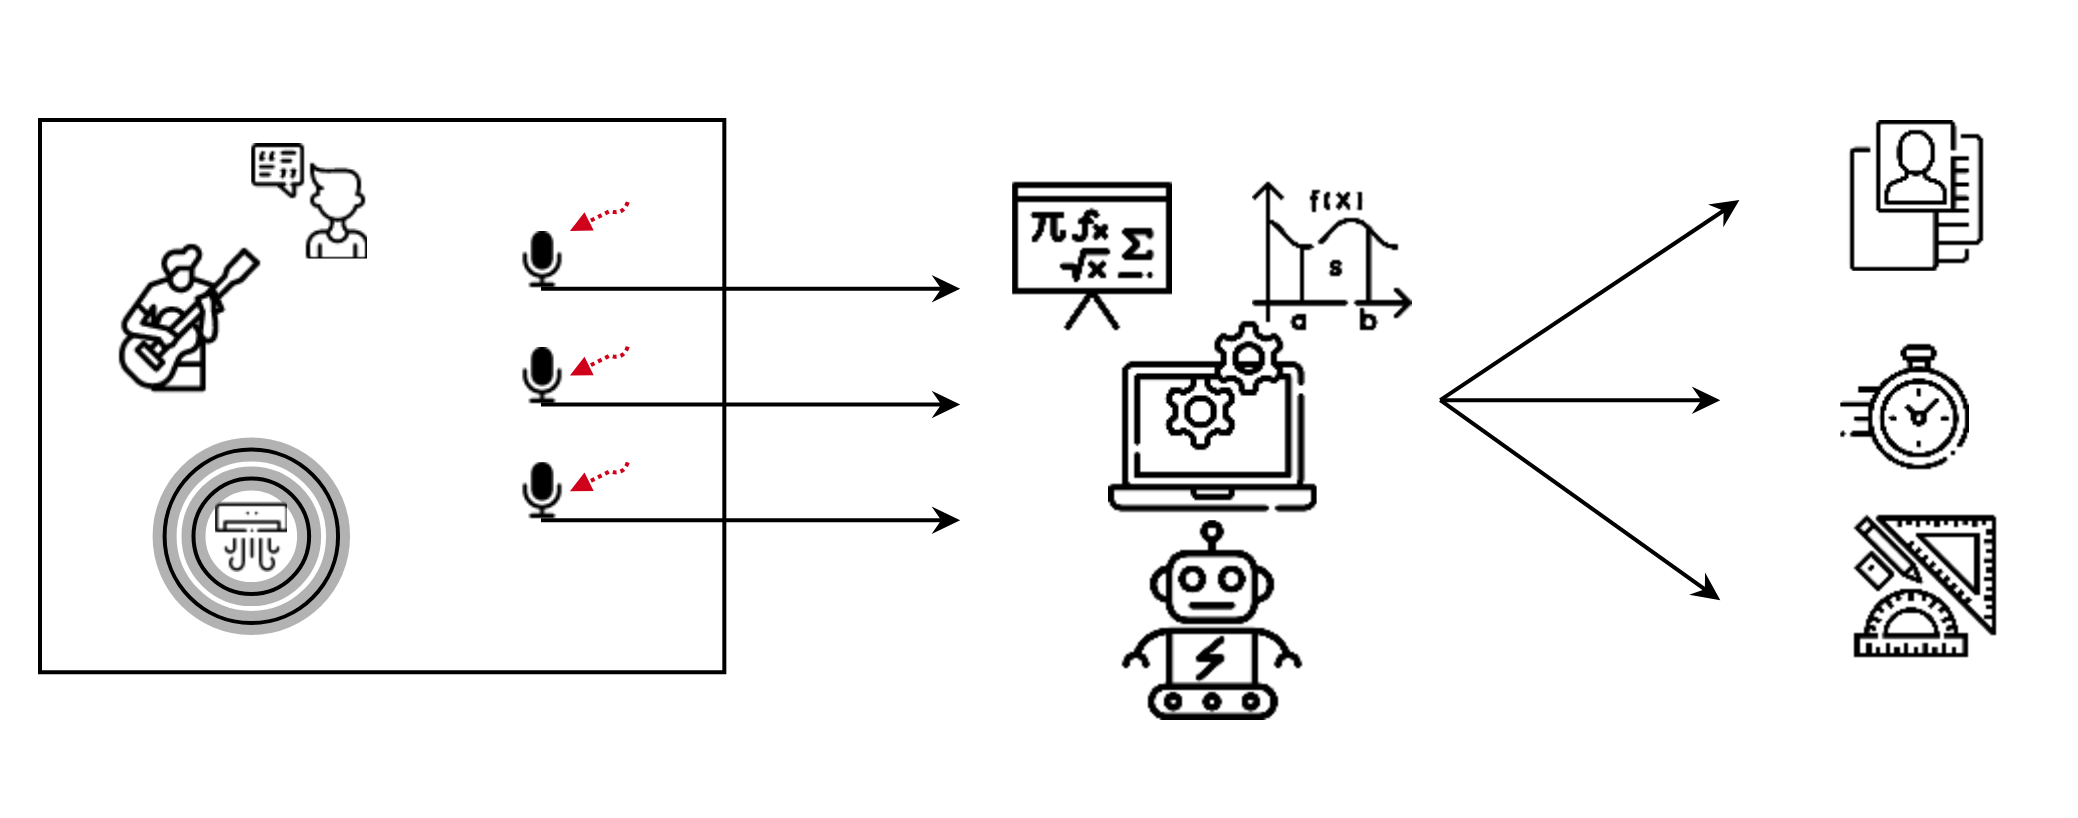
\includegraphics[trim={0 35mm 0 35mm},clip,width=0.8\textwidth]{figures/scene_analysis.png}
    \end{center}
    }

    \only<5->{
    \begin{textblock*}{40mm}(80mm,90mm)
        \textcolor{myred}{\textbf{Can computer do it?}}
    \end{textblock*}
    }

\end{frame}

\begin{frame}[t]{Echo-aware \alert{signal processing} for audio scene analysis}

    \begin{center}
        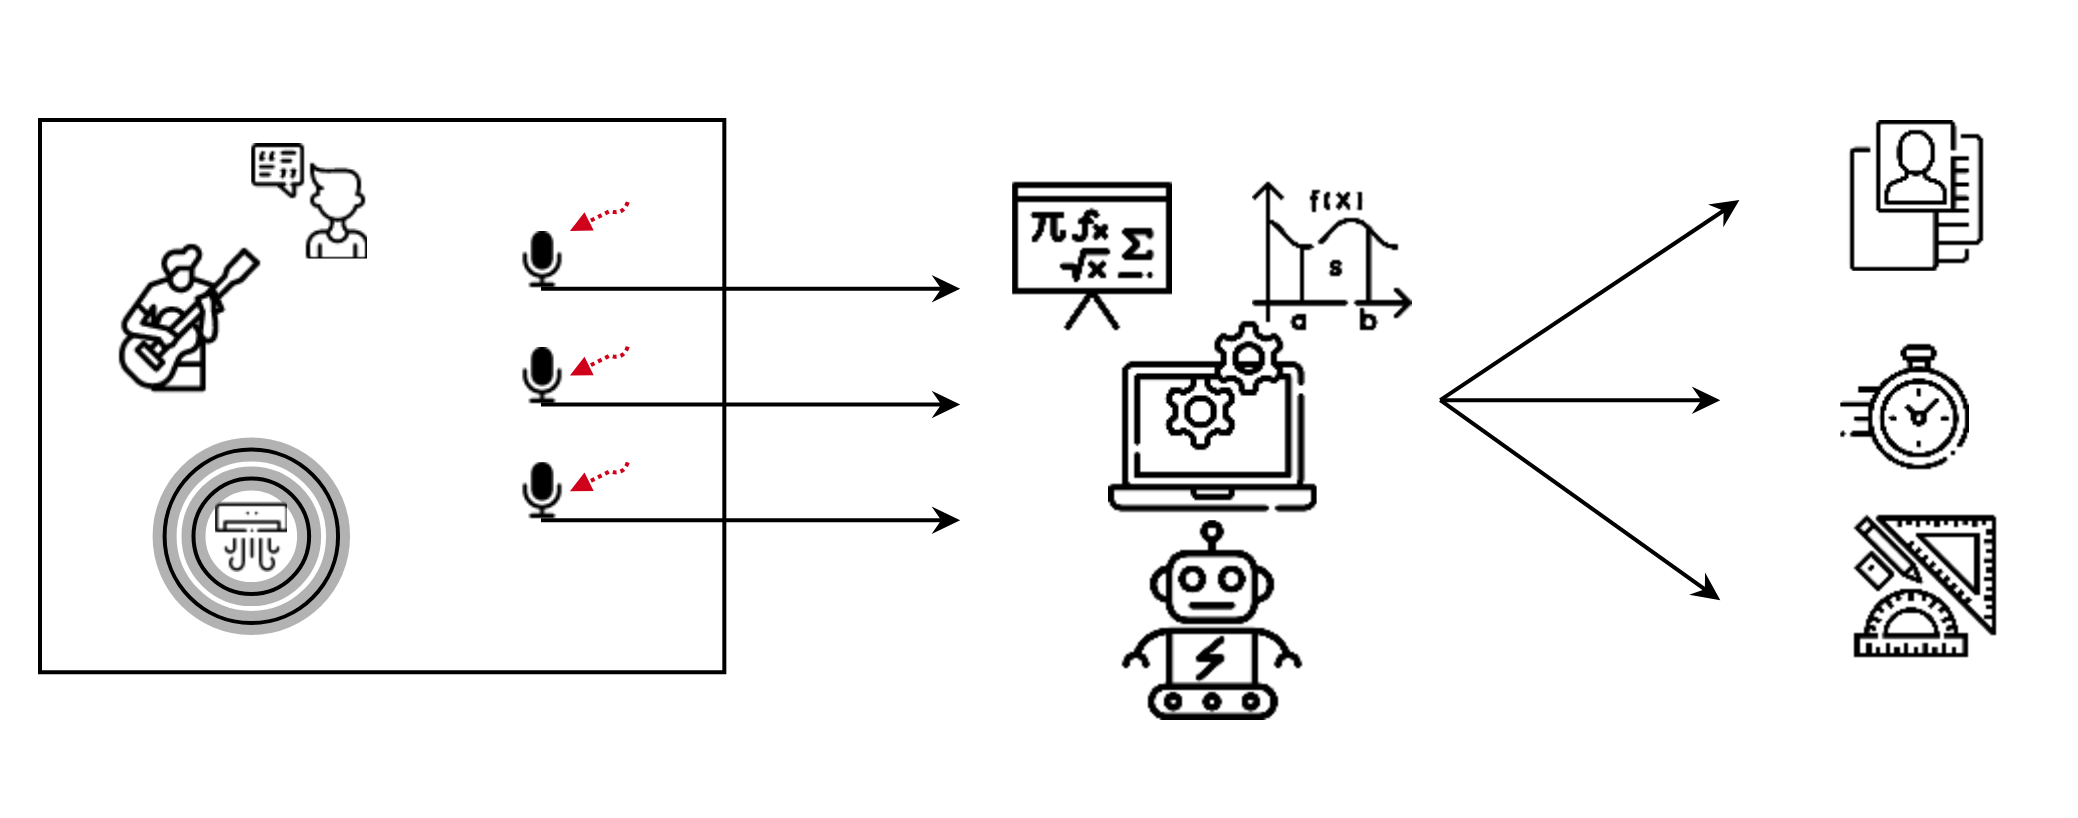
\includegraphics[trim={0 35mm 0 35mm},clip,width=0.8\textwidth]{figures/scene_analysis.png}
    \end{center}

    \pause
    \begin{mydefblock}{Signal Processing}
        Mathematical models, frameworks and tools to tackle and solve such problems
    \end{mydefblock}

    \pause
    {\small Some (inverse) problems}
    \begin{columns}[T,onlytextwidth]
        \begin{column}{0.48\textwidth}
            \begin{itemize}
                \item Speaker Identification\tikzmark{top1}\tikzmark{bot1}
                \item Sound Source Separation (SSS) \tikzmark{top2}
                \item Speech Enhancement (SE)
                \item Automatic Speech Recognition (ASR)\hspace{0.5em}\tikzmark{right1}\tikzmark{bot2}
                \item Sound Source Localization (SSL) \tikzmark{top3}
                \item Room Geometry Estimation (RooGE)  \tikzmark{bot3}
            \end{itemize}
        \end{column}

        \begin{column}{0.48\textwidth}
            \begin{itemize}
                \item Voice Activity Detection\tikzmark{top4}
                \item Diarization                \tikzmark{bot4}
                \item RT$_{60}$ estimation       \tikzmark{top5}
                \item Acoustic Channel Estimation\hspace{0.5em}\tikzmark{right2}
                \item Wall Absorption Estimation\tikzmark{bot5}
                \item \textit{and many many other}
            \end{itemize}

        \end{column}
    \end{columns}

    % \pause
    % \begin{tikzpicture}[overlay, remember picture]
    %     \node[anchor=base] (a) at (pic cs:top1) {\vphantom{h}}; % push the mark to the top of the line (ie including ascenders)
    %     \node[anchor=base] (b) at (pic cs:bot1) {\vphantom{g}}; % push the mark to the bottom of the line (ie including descenders)
    %     \draw [decoration={brace,amplitude=0.5em},decorate,thick,gray]
    %      (a.north -| {pic cs:right1}) -- node[right,inner sep=1em] {\small Who?} (b.south -| {pic cs:right1});
    % \end{tikzpicture}
    % \begin{tikzpicture}[overlay, remember picture]
    %     \node[anchor=base] (a) at (pic cs:top2) {\vphantom{h}}; % push the mark to the top of the line (ie including ascenders)
    %     \node[anchor=base] (b) at (pic cs:bot2) {\vphantom{g}}; % push the mark to the bottom of the line (ie including descenders)
    %     \draw [decoration={brace,amplitude=0.5em},decorate,thick,gray]
    %      (a.north -| {pic cs:right1}) -- node[right,inner sep=1em] {\small What?} (b.south -| {pic cs:right1});
    % \end{tikzpicture}
    % \begin{tikzpicture}[overlay, remember picture]
    %     \node[anchor=base] (a) at (pic cs:top3) {\vphantom{h}}; % push the mark to the top of the line (ie including ascenders)
    %     \node[anchor=base] (b) at (pic cs:bot3) {\vphantom{g}}; % push the mark to the bottom of the line (ie including descenders)
    %     \draw [decoration={brace,amplitude=0.5em},decorate,thick,gray]
    %      (a.north -| {pic cs:right1}) -- node[right,inner sep=1em] {\small Where?} (b.south -| {pic cs:right1});
    % \end{tikzpicture}
    % \begin{tikzpicture}[overlay, remember picture]
    %     \node[anchor=base] (a) at (pic cs:top4) {\vphantom{h}}; % push the mark to the top of the line (ie including ascenders)
    %     \node[anchor=base] (b) at (pic cs:bot4) {\vphantom{g}}; % push the mark to the bottom of the line (ie including descenders)
    %     \draw [decoration={brace,amplitude=0.5em},decorate,thick,gray]
    %      (a.north -| {pic cs:right2}) -- node[right,inner sep=1em] {\small When?} (b.south -| {pic cs:right2});
    % \end{tikzpicture}
    % \begin{tikzpicture}[overlay, remember picture]
    %     \node[anchor=base] (a) at (pic cs:top5) {\vphantom{h}}; % push the mark to the top of the line (ie including ascenders)
    %     \node[anchor=base] (b) at (pic cs:bot5) {\vphantom{g}}; % push the mark to the bottom of the line (ie including descenders)
    %     \draw [decoration={brace,amplitude=0.5em},decorate,thick,gray]
    %      (a.north -| {pic cs:right2}) -- node[right,inner sep=1em] {\small How?} (b.south -| {pic cs:right2});
    % \end{tikzpicture}

    \pause
    \vspace{-2mm}
    \begin{center}
        HOW  $\overset{\text{helps}}{\longrightarrow}$ WHERE
             $\overset{\text{helps}}{\longrightarrow}$ WHEN
             $\overset{\text{helps}}{\longrightarrow}$ WHAT
             $\overset{\text{helps}}{\longrightarrow}$ HOW
             $\overset{\text{helps}}{\longrightarrow}$ ...
    \end{center}

\end{frame}


\begin{frame}[t]{\alert{Echo-aware} signal processing for audio scene analysis}

    \begin{block}{Sound interacts with indoor environment:}
        \begin{itemize}
            \item[] it is reflected,\hspace{1em}\tikzmark{rightA}\tikzmark{topA}
            \\\hspace{1em} specularly and diffusely
            \item[$+$] it is absorbed,
            \item[$+$] it is transmitted,
            \item[$+$] and other.\tikzmark{botA}
        \end{itemize}
    \end{block}

    \begin{tikzpicture}[overlay, remember picture]
        \node[anchor=base] (a) at (pic cs:topA) {\vphantom{h}}; % push the mark to the top of the line (ie including ascenders)
        \node[anchor=base] (b) at (pic cs:botA) {\vphantom{g}}; % push the mark to the bottom of the line (ie including descenders)
        \draw [decoration={brace,amplitude=0.5em},decorate,thick,gray]
            (a.north -| {pic cs:rightA}) -- node[right,inner sep=1em]
                {$=$ all reverberation}
            (b.south -| {pic cs:rightA});
    \end{tikzpicture}

    \begin{mydefblock}{Acoustic Echoes}

        \vspace{-2mm}
        \begin{columns}[onlytextwidth]
            \begin{column}{0.60\textwidth}
                \begin{itemize}
                    \item Elements of reverberation
                    \item Specular reflection standing out for time and strength
                    \item Repetition of a sound but after
                    \begin{itemize}
                        \item same content
                        \item delay $\Leftrightarrow$ distance
                    \end{itemize}
                \end{itemize}
            \end{column}
            \begin{column}{0.38\textwidth}
                \centering
                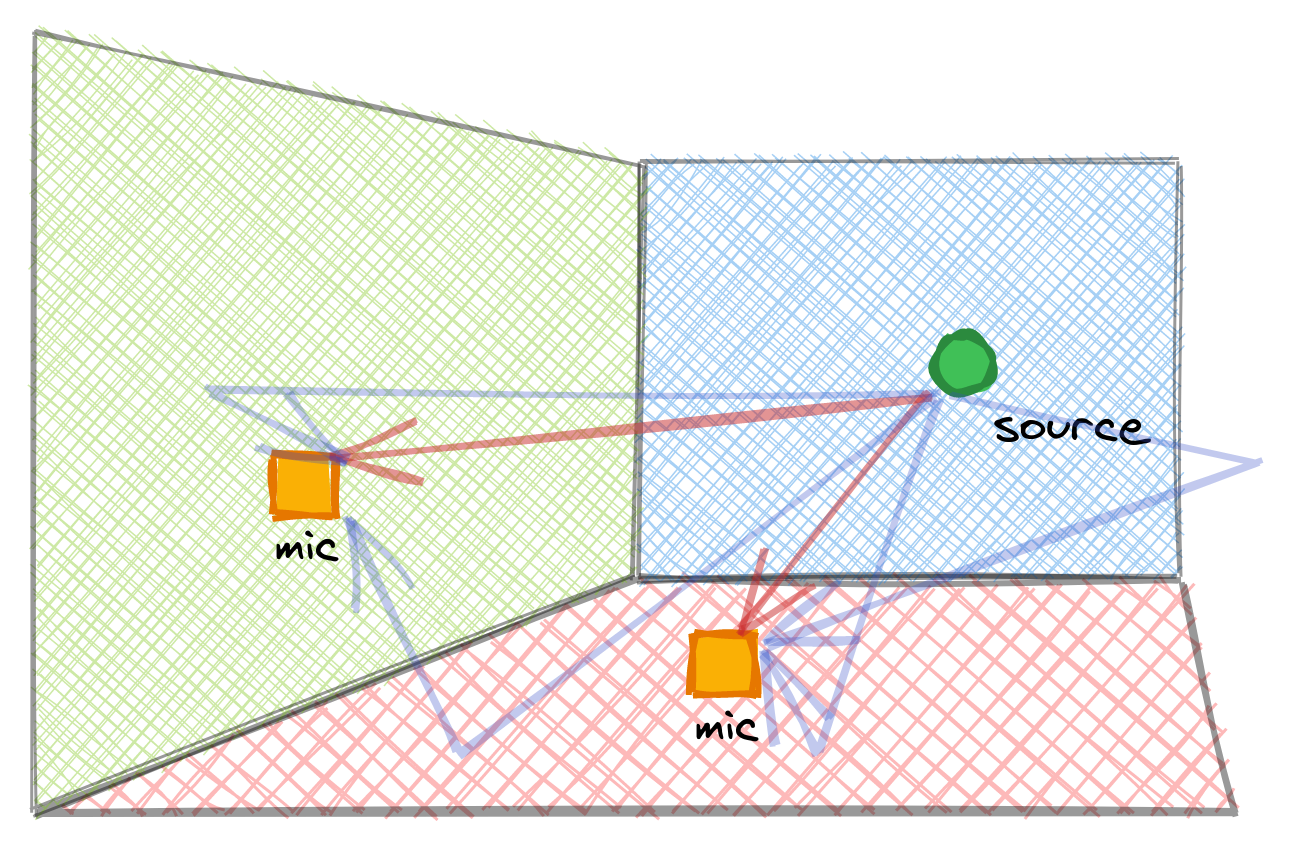
\includegraphics[width=.8\textwidth]{figures/echoes}
            \end{column}

        \end{columns}
    \end{mydefblock}

    \begin{block}{Everyday examples:}

        \vspace*{2mm}
        \begin{columns}[T,onlytextwidth]
            \column{.4\textwidth}
            Bat
            Dolphins
            Sonars
            \column{.22\textwidth}
            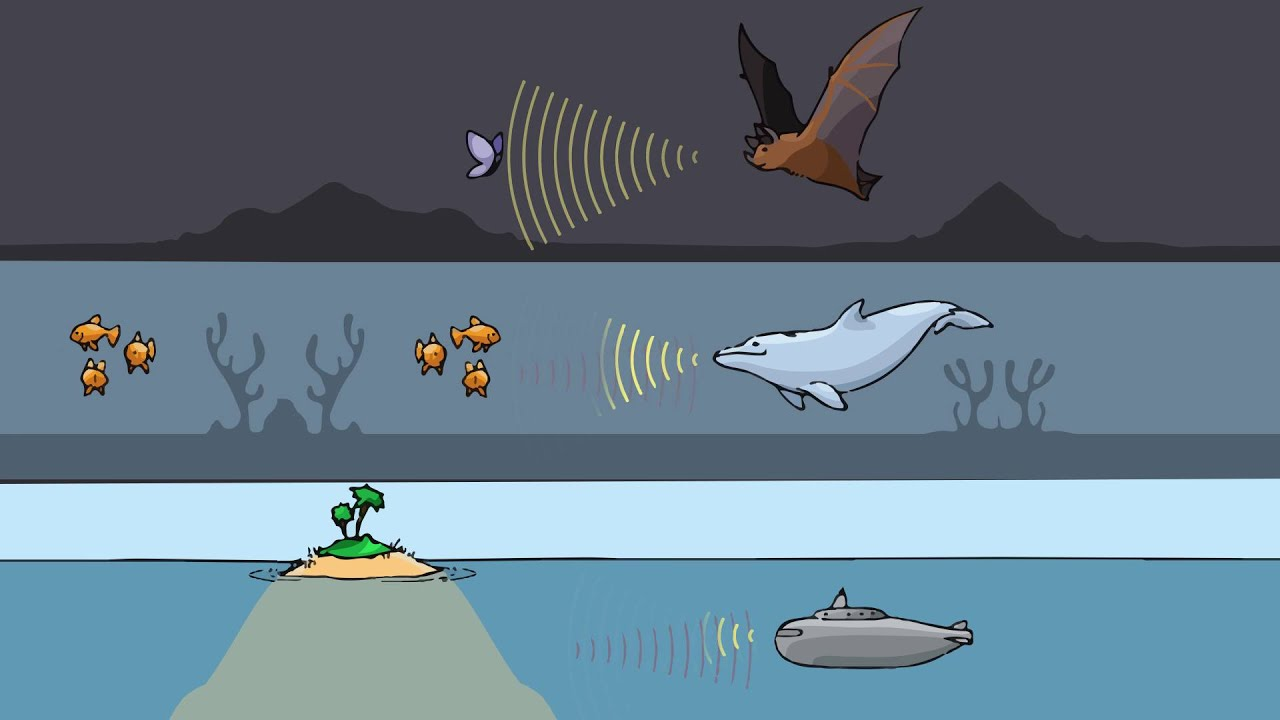
\includegraphics[width=\textwidth]{figures/echo_nature.jpg}
            \addendum{\small\faCopyright[regular]~Skin & Bones}
        \end{columns}
    \end{block}


    \begin{columns}
        \column{0.48\textwidth}
        Typically sound propagation is
        \begin{itemize}
            \item ignored $\implies$ simple processing but reverberation = noise
            \item fully modeled and estimated $\implies$ very challenging
        \end{itemize}

        \column{0.48\textwidth}
        \begin{mydefblock}{Echo-aware methods}
            Consider echoes for better processing
        \end{mydefblock}
    \end{columns}

\end{frame}

\subsection*{Outline and Contribution}

\begin{frame}{Outline and contributions}

    \begin{block}{Thesis title}

        \vspace*{2mm}
        \begin{columns}[onlytextwidth]
            \begin{column}[T]{0.3\linewidth}
                \centering
                \alert{Audio Scene Analysis}
                \\\downarrow
                \\context and problems
            \end{column}\hfill\pause
            \begin{column}[T]{0.3\linewidth}
                \centering
                \alert{Signal Processing}
                \\\downarrow
                \\models and frameworks
            \end{column}\hfill\pause
            \begin{column}[T]{0.3\linewidth}
                \centering
                \alert{Echo-aware}
                \\\downarrow
                \\better processing
            \end{column}\hfill
        \end{columns}
    \end{block}
    \pause

    \vfill
    \begin{block}{Thesis content:}

        \vspace*{2mm}
        \begin{columns}[T,onlytextwidth]
        \begin{column}{0.48\textwidth}
            \centering
            \alert{How to estimate them?}
            \begin{itemize}
                \item Analytical method
                \item Learning-based method
            \end{itemize}
            {\small no parameter tuning
            \\no full sound modeling}
        \end{column}
        \begin{column}{0.48\textwidth}
            \centering
            \alert{How to use them?}
            \begin{itemize}
                \item Source Localization
                \item Source Separation
                \item Speech Enhancement
                \item Room Geometry Estimation
            \end{itemize}
        \end{column}
    \end{columns}

    \begin{center}
        \alert{Where to find them?}
        \\Echo-aware database for
        \\estimation and application
    \end{center}
    \end{block}
\end{frame}